\documentclass[preview=true, border=10pt]{standalone}

\usepackage[compat=1.1.0]{tikz-feynman}

\newcommand{\GammaLoopsPenguinSize}{6.4}

\begin{document}
	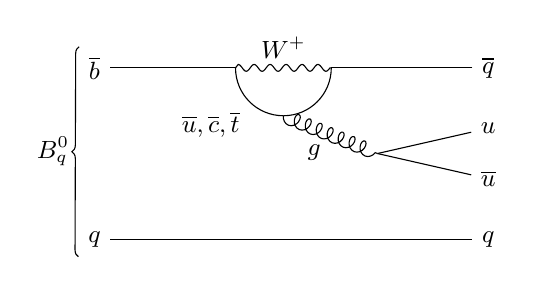
\begin{tikzpicture}
		\begin{feynman}
			\vertex (a1) {\small$\overline b$};
			\vertex[right=\GammaLoopsPenguinSize*0.28 cm of a1] (a2);
			\vertex[right=\GammaLoopsPenguinSize*0.19 cm of a2] (a3);
			\vertex[right=\GammaLoopsPenguinSize*0.28 cm of a3] (a4) {\small$\overline q$};
			\vertex[below=\GammaLoopsPenguinSize*0.34 cm of a1] (b1) {\small$q$};
			\vertex[below=\GammaLoopsPenguinSize*0.34 cm of a4] (b2) {\small$q$};
			\vertex at ($(a2)!0.5!(a3)!\GammaLoopsPenguinSize*0.095 cm!-90:(a3)$) (d);
			\vertex[below=\GammaLoopsPenguinSize*0.12 cm of a4] (c1) {\small$u$};
			\vertex[below=\GammaLoopsPenguinSize*0.10 cm of c1] (c3) {\small$\overline u$};
			\vertex at ($(c1)!0.5!(c3) - (\GammaLoopsPenguinSize*0.22 cm, 0)$) (c2);
			\diagram* {
			(a4) -- [plain] (a3) -- [boson, edge label'={\small$W^{+}$}] (a2) -- [plain] (a1),
			(b1) -- [plain] (b2),
			(c3) -- [plain] (c2) -- [plain] (c1),
			(a2) -- [plain, quarter right, edge label'={\small$\overline{u},\overline{c},\overline{t}$}] (d) -- [plain, quarter right] (a3),
			(d) -- [gluon, edge label'={\small$g$}] (c2),
			};
			\draw [decoration={brace}, decorate] (b1.south west) -- (a1.north west) node [pos=0.5, left] {\small$B_{q}^{0}$};
		\end{feynman}
	\end{tikzpicture}
\end{document}
